%%
%% This is file `pprbib.tex',
%% generated with the docstrip utility.
%%
%% The original source files were:
%%
%% ths.dtx  (with options: `pprbib')
%% 
%% IMPORTANT NOTICE:
%% 
%% For the copyright see the source file.
%% 
%% Any modified versions of this file must be renamed
%% with new filenames distinct from pprbib.tex.
%% 
%% For distribution of the original source see the terms
%% for copying and modification in the file ths.dtx.
%% 
%% This generated file may be distributed as long as the
%% original source files, as listed above, are part of the
%% same distribution. (The sources need not necessarily be
%% in the same archive or directory.)

 % ... preamble ...
\documentclass{article}

\usepackage[nopar]{lipsum}
\usepackage{graphicx}
\usepackage{threeparttable}
\usepackage{natbib}

\newcommand{\ThesisPaperAuthor}[1]{\title{#1}}
\newenvironment{ThesisPaperAbstract}{\begin{abstract}}{\end{abstract}}
\newcommand{\ThesisPaperKeywords}[1]{\textbf{Keywords:} #1}
\newenvironment{ThesisPaperBibliography}{}{}
\newcommand{\ThesisPaperReferences}[1]{\bibliography{#1}}

\begin{document}

 % ... title page ...

\ThesisPaperAuthor{%
 I.\ M.\ Author\\%
 Department of Mechanical \& Aerospace Engineering\\
 Missouri University of Science and Technology\\
 Rolla, Missouri 65409--0050\\
 Tel: 573--341--6622, Fax: 573--341--4115\\
 Email: imauthor@mst.edu%
}



 % ... abstract ...

\begin{ThesisPaperAbstract}
\lipsum[52-55]
\end{ThesisPaperAbstract}

 % ... keywords ...

\ThesisPaperKeywords{convection}

 % ... introduction ...

\section{Introduction}

\lipsum[52-55]

 % ... formulation ...

\section{Problem Formulation}%
  \label{sec:formulation}

\lipsum[56]
\subsection{Governing equations}

This is my simple equation
\begin{equation}
\delta_i = \sqrt{t/\mathrm{Pe}}
\end{equation}
where $\delta$ is the thermocline
thickness %
defined previously by \citep{bullwinkle.1990} and
\citet{bullwinkle.1991}. \lipsum[57-60]

Figure~\ref{fig:fig01} %
\begin{figure}[t]
  \begin{center}
  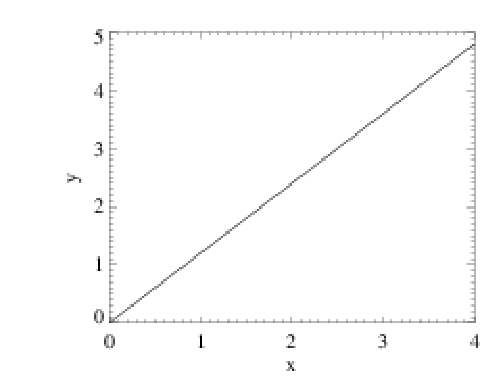
\includegraphics[width=3.75in]{simple.pdf}
  \end{center}
  \caption{The caption of the figure.}
\label{fig:fig01}
\end{figure}
illustrates the implementation of a very simple figure. \lipsum[61-65]

The inclusion of tables, such as Table~\ref{tbl:tbl01}, is just as
straigtforward. %
\begin{table}[t]
  \caption{THE CAPTION OF THE TABLE USES CAPITAL LETTERS.}
  \label{tbl:tbl01}
  \begin{center}
  \begin{tabular}{c l l}
  \hline
  Example & Time & Cost \\
  \hline
  1 & 12.5 & \$1,000 \\
  2 & 24 & \$2,000 \\
  \hline
  \end{tabular}
  \end{center}
\end{table}
Tables should appear in the order of their citation and should
generally appear at the top of the page in a final manuscript.
\lipsum[66-70]

 % ... results ...

\section{Results and Discussion} \label{sec:results}
\lipsum[71-80]

 % ... conclusions ...

\section{Conclusions}
\lipsum[81-85]

 % ... acknowledgments ...

\section*{Acknowledgments}
\lipsum[86]

 % ... references - bib files ...

\begin{ThesisPaperBibliography}{REFERENCES}
\bibliographystyle{plainnat}
\ThesisPaperReferences{add}
\end{ThesisPaperBibliography}

 % ... end ...

\end{document}


\endinput
%%
%% End of file `pprbib.tex'.
